\section{Russian dense delight}

Remember we ended the last post with a question: is it possible to associate with a prime~$p$ not dividing~$\Delta(f)$, an element~$\sigma_{p} \in G$ such that the decomposition type of~$f\bmod p$ is the same as the cycle type of~$\sigma_{p}$. I told you this could be done up to conjugacy, which I'll now explain. The element~$\sigma_{p}$ will be called the \emph{Frobenius substitution} of~$p$.

\subsection{Galois theory for finite fields}
The Frobenius, as an element of~$\Aut(\overline{\mathbb{F}}_{p})$, permutes the zeros of any polynomial with coefficients in~$\mathbb{F}_{p}$. For such a polynomial~$g$, the cycle pattern of the Frobenius, as a permution of the zeros of~$g$, is the same as the decomposition type of~$g$ over~$\mathbb{F}_{p}$. To see this, it's sufficient to suppose~$g$ irreducible, of degree~$n$ say. Then you know there is a root~$\alpha \in \mathbb{F}_{p^{n}}$, and that the other roots are~$\alpha^{p}, \alpha^{p^{2}},\ldots,\alpha^{p^{n-1}}$. The Frobenius obviously acts on~$g$ as the permutation~$(12\cdots n)$, and since~$g$ is irreducible, its decomposition type is also~$n$. Returning to the situation at hand, the statement we have just proven closely resembles the one in the introduction. To lift the Frobenius to a Frobenius substitution, which will be an element of~$\Aut(\mathbb{Q}(\alpha_{1},\ldots,\alpha_{d}))$, we'll need to connect the fields they're acting on. Notice that this means we want a way to reduce elements of~$\mathbb{Q}(\alpha_{1},\ldots,\alpha_{d})$ modulo~$p$. This is exactly what the notion of a \emph{place} will do for us.

\subsection{All over the place}
A place of~$\mathbb{Q}(\alpha_{1},\ldots,\alpha_{d})$ over~$p$ is a map~$\psi:\mathbb{Q}(\alpha_{1},\ldots,\alpha_{d}) \to \overline{\mathbb{F}}_{p}
\cup \{ \infty \}$, with the following properties:
\begin{enumerate}
  \item $\psi^{-1} \overline{\mathbb{F}}_{p}$ is a subring of~$\mathbb{Q}(\alpha_{1},\ldots,\alpha_{d})$, and~$\psi:\psi^{-1} \overline{\mathbb{F}}_{p} \to \overline{\mathbb{F}}_{p}$ is a ring morphism.
  \item $\psi(x)=\infty$ iff~$\psi(x^{-1})=0$, for an~$x \in \mathbb{Q}(\alpha_{1},\ldots,\alpha_{d})-\{0\}$.
\end{enumerate}

This is a concept frequently used in algebraic number theory, albeit in a different context. To motivate the definition a little, think about this as an extension of the classic reduction mod~$p$. Since~$p \equiv 0\bmod p$, it's only natural to introduce~$\infty$, since we would like~$1/p \equiv 1/0 \equiv \infty$. Taking the polynomial~$f$, and one of its roots~$\alpha_{1}$,~$\psi(f(\alpha_{1}))=0$. Since we would like a ring morphism, this would imply~$$\sum_{i=0}^{d} \overline{a_{i}} \psi(\alpha_{1})^{i}=0,$$ with~$f=\sum_{i=0}^{d} a_{i}X^{i}$, and~$a_{i} \in \mathbb{Z}$. This shows why the codomain has to contain~$\overline{\mathbb{F}}_{p}$.

\subsection{Frobenius substituion}

The places we have introduced have three important properties:
\begin{enumerate}
  \item a place of~$\mathbb{Q}(\alpha_{1},\ldots,\alpha_{d})$ over~$p$ exists, for every prime~$p$;
	\item if~$\psi$ and~$\psi’$ are two places over~$p$, then there is a~$\tau \in G$ such that~$\psi’=\psi \circ \tau$;
	\item if~$p \nmid \Delta(f)$, then~$\tau$ is unique.
\end{enumerate}
Taking a~$p \nmid \Delta(f)$, and~$\psi$ a place of~$K$ over~$p$, the map~$\psi'=\Frob \circ \psi$ is again a place, since~$\Frob$ is an~$\overline{\mathbb{F}}_{p}$-automorphism. If we apply property~$2$ to~$\psi$ and~$\psi'$, one finds a unique element~$\Frob_{\psi}$ in~$G$ such that~$\psi \circ \Frob_{\psi} = \Frob \circ \psi$. This element is going to be our Frobenius substitution. The end of the last paragraph showed us that the~$\psi(\alpha_{i})$ are the zeros of~$f\bmod p$ in~$\overline{\mathbb{F}}_{p}$, and the characterizing property of~$\Frob_{\psi}$ tells us that it permutes~$\alpha_{1},\ldots,\alpha_{d}$ in exactly the same way as~$\Frob$ permutes~$\psi(\alpha_{1}),\ldots,\psi(\alpha_{d})$. This means that the cycle pattern of~$\Frob_{\psi}$ is equal to the decomposition type of~$f\bmod p$.

There's no reason why~$\Frob_{\psi}$ shouldn't depend on the choice of place~$\psi$. Taking~$\eta$ to be another place over~$p$, we know by property~$2$ that~$\eta=\psi \circ \tau$, and thus
\begin{equation}
  \psi \circ \tau \circ \Frob_{\psi \circ \tau}=\Frob \circ\, \psi \circ \tau=\psi \circ \Frob_{\psi} \circ \tau. 
\end{equation}
Taking~$\Frob_{\psi \circ \tau}$ equal to~$\tau^{-1} \circ \Frob_{\psi} \circ \tau$ does the trick, and by property~$3$, it's unique. This means that~$\Frob_{\psi}$ ranges over a conjugacy class as~$\psi$ varies over all the places over~$p$. We'll denote a typical element of this conjugacy class by~$\sigma_{p}$.

\subsection{Chebotar\"ev density}

All of this allows for the formulation of the announced theorem
\begin{theorem}
  Let~$f$ be a monic polynomial with integer coefficients and nonzero discriminant~$\Delta(f)$. Let~$C$ be a conjugacy class of the Galois group of~$f$. Denote by~$S$ the following set,
  \begin{equation}
    S=\{ p\,|\, \text{$p$ prime}, p\nmid \Delta(f), \sigma_{p} \in C \}. 
  \end{equation}
  Then~$S$ has a density, which is equal to~$\vert C \vert / \vert G \vert$.
\end{theorem}

Let's see how exactly this generalizes our previous two theorems. First off, Dirichlet. The only thing we have to do in this case, is pick~$f$ to be equal to~$X^{m}-1$. Since the Galois group is abelian, the conjugacy classes are the elements, so choose~$a \in G \cong (\mathbb{Z}/m\mathbb{Z})^{*}$, and thus~$a$ coprime with~$m$. Now what is the unique element~$\sigma_{p}$? For~$\psi$ a place over~$p$, we know that~$\psi(\sigma_{p}(x))=\psi(x)^{p}$, for all~$x \in \mathbb{Q}(\zeta)$. Picking~$x$ to be~$\zeta$, and knowing that~$\sigma_{p}(\zeta)=\zeta^{a}$ (this is how you identify~$G$ with~$(\mathbb{Z}/m\mathbb{Z})^{*}$), we get that~$\psi(\zeta)^{a}=\psi(\zeta)^{p}$. Since~$\psi(\zeta)$ is a primitive~$m$-th root of unity, one has~$a \equiv p$ mod~$m$, and Dirichlet pops out.

The way it generalizes Frobenius is slightly trickier, since it needs a reformulation of Frobenius employing \emph{divisions of~$G$}. A division is sort of a conjugacy up to a power. Given an element~$g \in G$ of order~$m$, the division of~$g$ consists of all elements that are conjugate to any~$g^{n}$, as long as~$n$ and~$m$ are coprime. Obviously, a conjugacy class is part of a division. The converse isn't necessarily true; two element can belong to the same division without being conjugated. A simple abelian example is given by the elements~$3$ mod~$10$ and~$7$ mod~$10$, which aren't equal in~$\mathbb{Z}/10\mathbb{Z}$, and thus not conjugated, but~$7^{3}=3$, so they're in the same division. The alternative statement of Frobenius density then says exactly what Chebotar\"ev density says, with 'conjugacy class' replaced by 'division'. Often, Chebotar\"ev can distinguish between primes that get stuck together with Frobenius.

\subsection{Application}

I just can't let you go without a small, beautiful, and rather mysterious application of Chebotar\"ev. The statement is this:

\begin{corollary}
  If~$f \in \mathbb{Z}[X]$ is an irreducible polynomial that has a~$0$ modulo almost all primes, then~$f$ is linear.

  \begin{proof}
    Assume that~$\deg(f)>1$. Since the Galois group of~$f$ acts transitively on the roots~$\Omega$, and for almost all primes~$p$,~$f\bmod p$ has a zero in~$\mathbb{F}_{p}$, almost all Frobenius substitutions fix a root of~$f$. Taking~$S$ to be the set of all~$g \in G$ that fix at least one element of~$\Omega$, we see that
    \begin{equation}
      S=\bigcup_{\omega \in \Omega} \Stab(\omega)=\bigcup_{g \in G} g \Stab(x) g^{-1}, 
    \end{equation}
    with~$x$ a fixed element of~$\Omega$. The first equality is trivial; the second one as well, if you remember to use transitivity. Since no finite group is the union of conjugates of a proper subgroup,~$G$ has to contain elements that don't fix a root of~$f$. These elements can be the Frobenius subsitution of only finitely many primes, which is impossible by Chebotar\"ev, which says there should always should be a density, and we know a finite set has density~$0$.
  \end{proof}
\end{corollary}

\begin{wrapfigure}{r}{.35\textwidth}
  \centering
  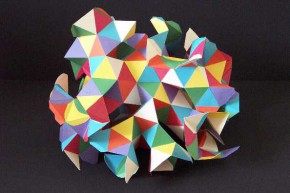
\includegraphics[width=.3\textwidth]{chebotarev-density/hyperbolic}
\end{wrapfigure}
Of course, one would also like a completely algebraic proof of the theorem, not requiring a big cannon like Chebotar\"ev (the proof of which uses lots of L-functions and complex analysis). The surprising thing is that the only known algebraic proofs make use of none other than the \emph{classification of finite simple groups}!

Let me just provide you with the glue that relates~$\mathbb{F}_{1}$-geometry to recreational number theory (my state of mind upon writing the first post seems not to have been overly optimistic):
\begin{quote}
  ``\textsl{Recreational number theory is that branch of number theory which is too difficult for serious study.}''
\end{quote}
By now I'm sure you can guess who it was that uttered this phrase.
